\documentclass[11pt,a4paper]{article}
\usepackage[utf8]{inputenc}
\usepackage[margin=1in]{geometry}
\usepackage{titlesec}
\usepackage{enumitem}
\usepackage{hyperref}
\usepackage{xcolor}
\usepackage{graphicx}
\usepackage{subcaption}
\usepackage{graphicx}
\usepackage{float}

\titleformat*{\subsection}{\bfseries\color{tuedark}}
% --- Custom Styling for Academic Polish ---
\definecolor{tuedark}{HTML}{1E293B}
\definecolor{tuegreen}{HTML}{16A34A}

\titleformat*{\section}{\large\bfseries\color{tuedark}}
\titleformat*{\subsection}{\boldseries\color{tuedark}}
\titleformat*{\subsection}{\bfseries\color{tuedark}}
\hypersetup{
    colorlinks=true,
    linkcolor=tuedark,
    urlcolor=tuegreen,
    citecolor=tuegreen
}

% --- Cover/Metadata Setup ---
\title{\textbf{Phase 2 Final Report:\\ AI-Supported Sustainability Self-Assessment for TU/e Research}}

\author{\textbf{Group Q} \\\\
Course: 5ARF0 Ethics of AI: Theory and Practice \\
Eindhoven University of Technology}
\date{\today}


\begin{document}

\maketitle
\vspace{1cm}

\thispagestyle{empty}
\clearpage
\pagestyle{plain}
=
% A. PROJECT TITLE
% =========================================================================
\section*{A. Project Title}
\addcontentsline{toc}{section}{A. Project Title}

\noindent\textbf{Research Roots: Finding Related TU/e Research and Reusable Resources}
% =========================================================================
% B. PUBLIC SUMMARY
% =========================================================================
\section*{B. Public Summary}
\addcontentsline{toc}{section}{B. Public Summary}


\vspace{1em}
\noindent Our AI-Supported Sustainability Self-Assessment for TU/e Research (ENSU) project handles how TU/e university researchers can check the hidden environmental footprints of localized laboratory or computational experiments. It presents an interactive, self-assessment web application that helps users to build layout guides using an integrated large language model (LLM). On the other hand, a separate step-by-step calculation tool checks resource consumption measurements like equipment runtime, electricity use, e.t.c. This tool is crucial for TU/e stakeholders and the public as it successfully transforms high-level campus sustainability goals into mindful day-to-day operations for researchers. To further sweeten the pot, the whole process of using this tool is done without strict rules or paperwork getting in the way.\\ 

The major anticipated challenges include;\\ 1) Defining clear assessment boundaries for shared laboratory equipment or infrastructure.\\ 2) Ensuring complete traceability of all provided recommendations and finally,\\ 3) Preventing users from becoming overreliant on automated feedback.
\clearpage

% =========================================================================
% C. COMPREHENSIVE SUMMARY
% =========================================================================
\section*{C. Comprehensive Summary}
\addcontentsline{toc}{section}{C. Comprehensive Summary}

\subsection*{Problem Definition and Objective(s)}

A student starting a new project may find a paper on the same topic, but still miss a useful method or piece of equipment in another TU/e department. The university's research portal already has projects, publications and equipment (TU/e, n.d.-a). The difficulty we want to explore is what happens before the student knows the right title, author or search term. We do not yet know how often this is a problem at TU/e, so we would check it with researchers instead of presenting it as a proven gap.

We propose a website where a student or researcher enters a short description of a planned study: the question, method and, if relevant, equipment needed. The site would show related TU/e work and explain the connection. For example, someone planning a LiDAR experiment might find a similar sensing method used for a different purpose in another department. They could then ask whether a protocol, dataset or setup can be reused. This may save time and resources, but finding a match does not itself save electricity or materials. We would test whether people actually change their plans after using the site.

The main users would be students and researchers at an early planning stage. Project leaders might use it to find partners. Librarians, equipment managers and data stewards would help keep records useful and decide what can be shared. Researchers whose projects appear in the results should be able to decide whether details of unfinished work are visible. The tool would support their judgment; it would not decide whether a project is original or deserves funding. Contacting another group can also create work for that group. The site should help users decide when a conversation is worthwhile rather than send automatic requests to everyone with a similar project.

\subsection*{Background of Current Approaches and Knowledge}

The TU/e portal is the obvious starting point. We would build on records that the university allows us to reuse rather than create a second collection from scratch. Public indexes such as OpenAlex could give some wider context for published work (OpenAlex, 2026). Neither source, however, tells us about every ongoing project or confidential idea. For an initial version, we would use permitted titles, abstracts and equipment descriptions. A researcher could also choose to add a short summary of work in progress. Every result would show where it came from and when it was last updated.

Existing research gives us a reason to look for connections, but it does not tell us exactly what TU/e researchers need. In one study at a US university, later collaboration was most common when researchers had some topic overlap, rather than almost none or almost complete overlap (Smith et al., 2021). A study including TU/e also argues that sustainability work depends on cooperation across departments and on support from the university (Karo et al., 2026). These findings suggest possible benefits, yet we still need to ask local users when they welcome a match and when it might feel like competition or unwanted exposure.

There are also technical methods worth trying. Models such as SPECTER compare scientific texts using titles, abstracts and citation links (Cohan et al., 2020). Later work shows that performance differs between search and ranking tasks (Singh et al., 2023). We therefore cannot assume that an embedding model will understand short project plans well. We would compare it with ordinary keyword search and ask researchers whether the suggested links make sense. We would record our search terms, sources and selection decisions so that the background review can be checked. For example, a sensing method might appear in robotics and building research under different keywords. A method-based link could reveal this, though a researcher still has to decide whether the technique really transfers.

\subsection*{Plan of Approach / Design Strategy}

We will use Value Sensitive Design as a way to ask whose needs the site serves and how its features affect them (Friedman et al., 2008). The main values we have identified are sustainability, privacy, fairness, researchers' control over their ideas and explicability. Explicability matters here because a user needs to see why two projects were linked. Privacy matters because a brief project description can reveal an unpublished direction. Fairness matters if one department has more complete records and therefore appears more often in results. These are our starting points, not a final list chosen on behalf of users.

First, we would speak with researchers from different departments, a librarian or research-support worker, and a data steward. We would ask how they currently find related work, what makes a match useful, and which details they would be willing to share. A simple mock-up would help them react to something concrete. Their comments would shape the required fields, sharing options and explanations. TU/e requires ethical review for research with participants or personal data, so any interviews or user tests would follow the relevant procedure (TU/e, n.d.-b).

The first prototype would ask for a short description of the problem, method and possible application. It would search permitted records by keywords and by scientific-text similarity. A user could say whether topic, method or equipment is most important. Results would be grouped under these headings, with a link back to the original record. We would avoid presenting one exact similarity percentage, since the same number could hide different kinds of connection. If an abstract is missing or a department is poorly covered, the site should say so. We would use a compact search method first and add generated wording only if users understand the results better without extra errors or unreasonable computing costs.

The proposed interface has three linked trees. A \emph{similarity tree} shows which records share a topic, method or resource with the user's idea. A \emph{difference tree} points out how the idea differs from the records found; it cannot prove that the difference is a new research gap. A \emph{future tree} gives questions the researcher could discuss with a supervisor, based on the same records. Each branch should lead to its source. Users could mark a bad match, save a useful one or ask for contact through an approved channel. The tree design is meant to make the information easier to explore; a tree image alone is not evidence of sustainability.

A user's draft description would not automatically join the shared database. They could separately agree to share a short summary, choose who may see it and later withdraw it. TU/e staff would have to approve storage, access and maintenance arrangements under the university's research-data policy (TU/e, n.d.-c). Someone must also correct outdated records and answer complaints about wrong links. Without this work, even a good search model would soon become less useful.

We would begin with a small set of records from two departments and review missed matches with researchers before expanding it. That would let us check permissions and record quality without assuming that one method works equally well across the university. We would then test the prototype with tasks drawn from real project-planning situations. Users would try both the current portal and the new interface. We would ask domain experts to judge whether the top matches are relevant and whether the explanations are accurate. We would measure time to find a useful record or contact and note where users correct or reject a suggestion. Later, we would ask whether a match led to a conversation, reuse of data or equipment, or a changed plan. Those actions are closer to our goal than clicks. Any estimate of saved resources would need a clear comparison case and would include the site's own computing costs. This is the path by which the tool might help environmental sustainability, but its effect remains to be shown.

\subsection*{Comparison to Alternatives}

Our Phase 1 idea was an AI-supported self-assessment of a research activity's environmental footprint. That could be useful once a workflow is defined, but it needs measurements and reference data. The new idea acts earlier, while the researcher can still choose a method or reuse an existing resource. A simpler option would be to improve the current portal's search filters without AI. We would keep that as the baseline; if semantic matching does not help users find better results, the simpler option is preferable.

The main challenges are incomplete records, different terms across fields, confidential work and misleading matches. A polished tree might make a weak suggestion look certain. We would show sources and missing information and let researchers correct results. We also need to avoid implying that similar work makes a new project pointless: a similar method can serve a different question. The aim for this phase is a design that can be tested honestly, not a claim that the website has already reduced research waste.

% =========================================================================
% D. RESPONSIBLE INNOVATION PROJECT STATEMENT
% =========================================================================
\section*{D. Responsible Innovation Project Statement}
In the responsible innovation statement we will assess our tool on different ethical principles. The use of AI raises concerns in terms of transparency, bias and reliability. We will discuss these concerns and provide measures to make sure our tool is in line with the users’ values. \newline

The first concern is the transparency of the tool. From the users perspective they submit their research into the tool and receive potentially previous done research on their topic. The user does not always know why the sources provided are relevant and whether the information provided by the AI is correct. The following measures will be taken:\newline
Source transparency: Every source provided by the tool will need to include title authors year of publication the link to the original source and additional information if possible. This way the researches can verify the sources instead of having to trust the AI\newline
Explanation of relevance: For each source provided a short explanation needs to be included on why the source was provided by showing similarities in research questions, methods etcetera. \newline

Depending on the available sources the Ai can be a bit biased. Especially if it only has access to certain types of sources like journals or only English sources. This could result in researchers missing previously conducted research when the tool does not have access to these sources. Our tool will try to prevent the bias as much as possible with the following measures: \newline
Database coverage: it should be clear for the user which databases the tool has access to. This way the user knows the limitations of the tool.
Search strategies: If possible the AI should make a broad search by using synonyms, interdisciplinary similarity and different terminology. \newline 
User input: The user should be able to adjust the search query if they feel like it could be improved giving them more control over the results in case the AI runs into limitations. \newline

Our main design is to make it easy for the users to interpret the results by having a chatbot that provides the sources and explains why the sources are relevant. In future work we could help researches by providing improvements on their research. Even when there is research on the same topic there are still ways to differentiate. This way the researcher does not have to scrap everything and still conduct useful research. The tool could provide a better use of the resources for the research in case this happens. 


% =========================================================================
% E. REFERENCE LIST
% =========================================================================
\section*{E. Reference List}
\addcontentsline{toc}{section}{E. Reference List}

\begin{thebibliography}{99}

\bibitem[Cohan et~al.(2020)]{cohan2020}
Cohan, A., Feldman, S., Beltagy, I., Downey, D., \& Weld, D. S. (2020).
SPECTER: Document-level representation learning using citation-informed transformers.
\emph{Proceedings of the 58th Annual Meeting of the Association for Computational Linguistics}, 2270--2282.
\url{https://doi.org/10.18653/v1/2020.acl-main.207}

\bibitem[Friedman et~al.(2008)]{friedman2008}
Friedman, B., Kahn, P. H., Jr., \& Borning, A. (2008).
Value sensitive design and information systems.
In K. E. Himma \& H. T. Tavani (Eds.), \emph{The handbook of information and computer ethics}. Wiley.
\url{https://doi.org/10.1002/9780470281819.ch4}

\bibitem[Karo et~al.(2026)]{karo2026}
Karo, E., Shakya, S., Voll, C. N., Fuchs, L., Cuevas Garcia, C., \& Lember, V. (2026).
How can universities become transformative change agents? Sustainability strategizing in European technological universities.
\emph{Minerva}.
\url{https://doi.org/10.1007/s11024-026-09636-z}

\bibitem[OpenAlex(2026)]{openalex2026}
OpenAlex. (2026).
\emph{Works overview}.
\url{https://help.openalex.org/data/works/}

\bibitem[Singh et~al.(2023)]{singh2023}
Singh, A., D'Arcy, M., Cohan, A., Downey, D., \& Feldman, S. (2023).
SciRepEval: A multi-format benchmark for scientific document representations.
\emph{Proceedings of the 2023 Conference on Empirical Methods in Natural Language Processing}, 5548--5566.
\url{https://doi.org/10.18653/v1/2023.emnlp-main.338}

\bibitem[Smith et~al.(2021)]{smith2021}
Smith, T. B., Vacca, R., Krenz, T., \& McCarty, C. (2021).
Great minds think alike, or do they often differ? Research topic overlap and the formation of scientific teams.
\emph{Journal of Informetrics, 15}(1), 101104.
\url{https://doi.org/10.1016/j.joi.2020.101104}

\bibitem[TU/e(n.d.-a)]{tueportal}
Eindhoven University of Technology (TU/e). (n.d.-a).
\emph{Research portal}.
\url{https://research.tue.nl/en/}

\bibitem[TU/e(n.d.-b)]{tueethics}
Eindhoven University of Technology (TU/e). (n.d.-b).
\emph{Ethical approval}.
\url{https://rdm.tue.nl/docs/before-research/ethical-approval/}

\bibitem[TU/e(n.d.-c)]{tuerdm}
Eindhoven University of Technology (TU/e). (n.d.-c).
\emph{TU/e RDM framework policy}.
\url{https://rdm.tue.nl/docs/intro/tue-policy/}

\end{thebibliography}

\clearpage
% =========================================================================
% F. USER NARRATIVE
% =========================================================================
\section*{F. User Narrative}
\addcontentsline{toc}{section}{F. User Narrative}

\noindent Dr. Alex, a postdoctoral researcher at Eindhoven University of Technology, is designing a new fabrication run of lithium-ion battery electrode samples within a TU/e laboratory building. Eager to lower total electricity and material waste without changing the scientific parameters that make the batch valid, Alex logs onto the AI-Supported Sustainability Self-Assessment (ENSU) web portal from his laptop or phone.\\

On the home dashboard, Alex selects "1. I want to Assess", initiating a 5-step evaluation process. Rather than selecting rigid checkboxes, Alex inputs a plain-text description: "I make lithium-ion battery electrode samples. I want to minimize material loss and electricity use while preserving our existing electrochemical testing requirements." The system’s hidden language model parses the text and displays a unique suggestion box: "This appears to be a laboratory battery-sample activity." Alex clicks "Confirm activity", advancing to the data input sheet.\\

Alex completes the project fields based on a prior set of data: 6 fabrication attempts yielding 5 valid samples, consuming 60 kWh of meter-tracked laboratory electricity and 1.2 kg of starting materials. The system asks a follow-up question regarding what constitutes a valid sample. Alex types: "A valid sample passes our electrochemical test and safety checks."\\

Upon confirming the fields, the tool runs its sep-by-step engine and outputs an initial evaluation profile. Rather than showing an aggregated green score or compliance badge, the interface reports isolated multi-dimensional measurements: an active resource footprint of 12 kWh per valid sample, leaving a 2 kWh gap above Alex's personal sustainability target of 10 kWh. Beneath the values, a targeted suggestion appears: "Pilot a process change that reduces failed samples; record electricity, starting material, valid samples, and test results for the whole batch." Alex clicks "Plan pilot", exits the interface, and carries out the optimized process in the lab.\\

A week later, Dr. Alex returns to the ENSU web portal. He navigates to "My History" under the "Query" module, and logs the pilot outcomes: 6 attempts, 6 valid samples, 54 kWh, and 1.1 kg of material. The comparison dashboard updates instantly, using smooth visual bar meters to track the positive project shift: batch electricity dropped by 6 kWh, material consumption fell by 0.1 kg, and efficiency reached 9 kWh per sample, thereby cleanly surpassing Dr. Alex's original goal. Alex saves the session privately to the(his) personal archive, double-checking a research plan step-by-step through transparent data reflection.



\section*{G. Visual Representation of Mock-up}
\addcontentsline{toc}{section}{G. Visual Representation of Mock-up}

\begin{figure}[H]
    \centering
    % Row 1
    \begin{subfigure}{0.48\linewidth}
        \centering
        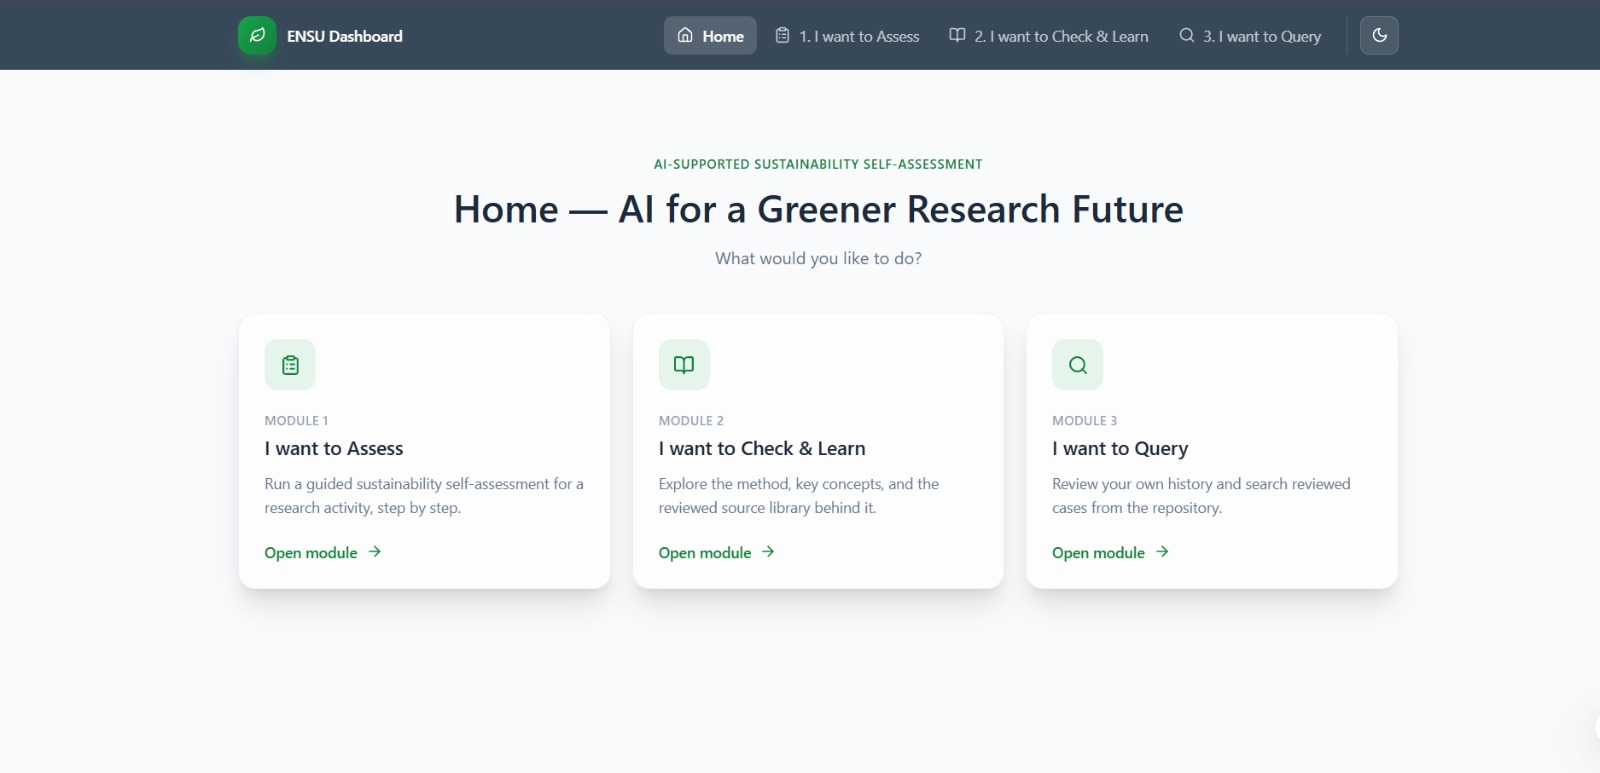
\includegraphics[width=\linewidth]{LaTeX_tuemscthesis2021/1.jpeg}
        \caption{Home page - Light Mode}
    \end{subfigure}
    \hfill
    \begin{subfigure}{0.48\linewidth}
        \centering
        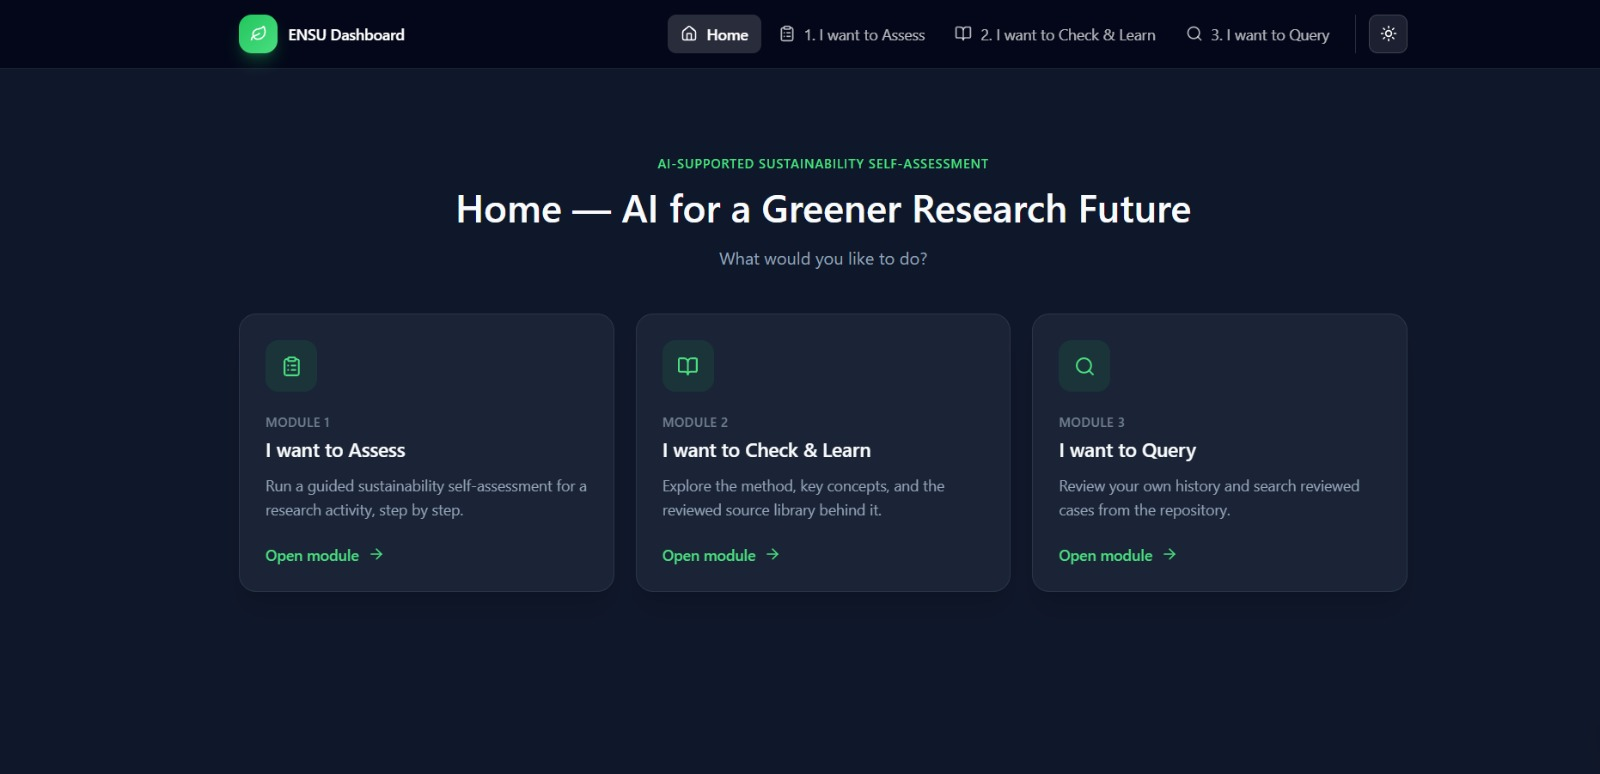
\includegraphics[width=\linewidth]{LaTeX_tuemscthesis2021/2.jpeg}
        \caption{Home page - Dark Mode}
    \end{subfigure}

    \vspace{0.3cm} % Tightly controls vertical spacing between rows

    % Row 2
    \begin{subfigure}{0.48\linewidth}
        \centering
        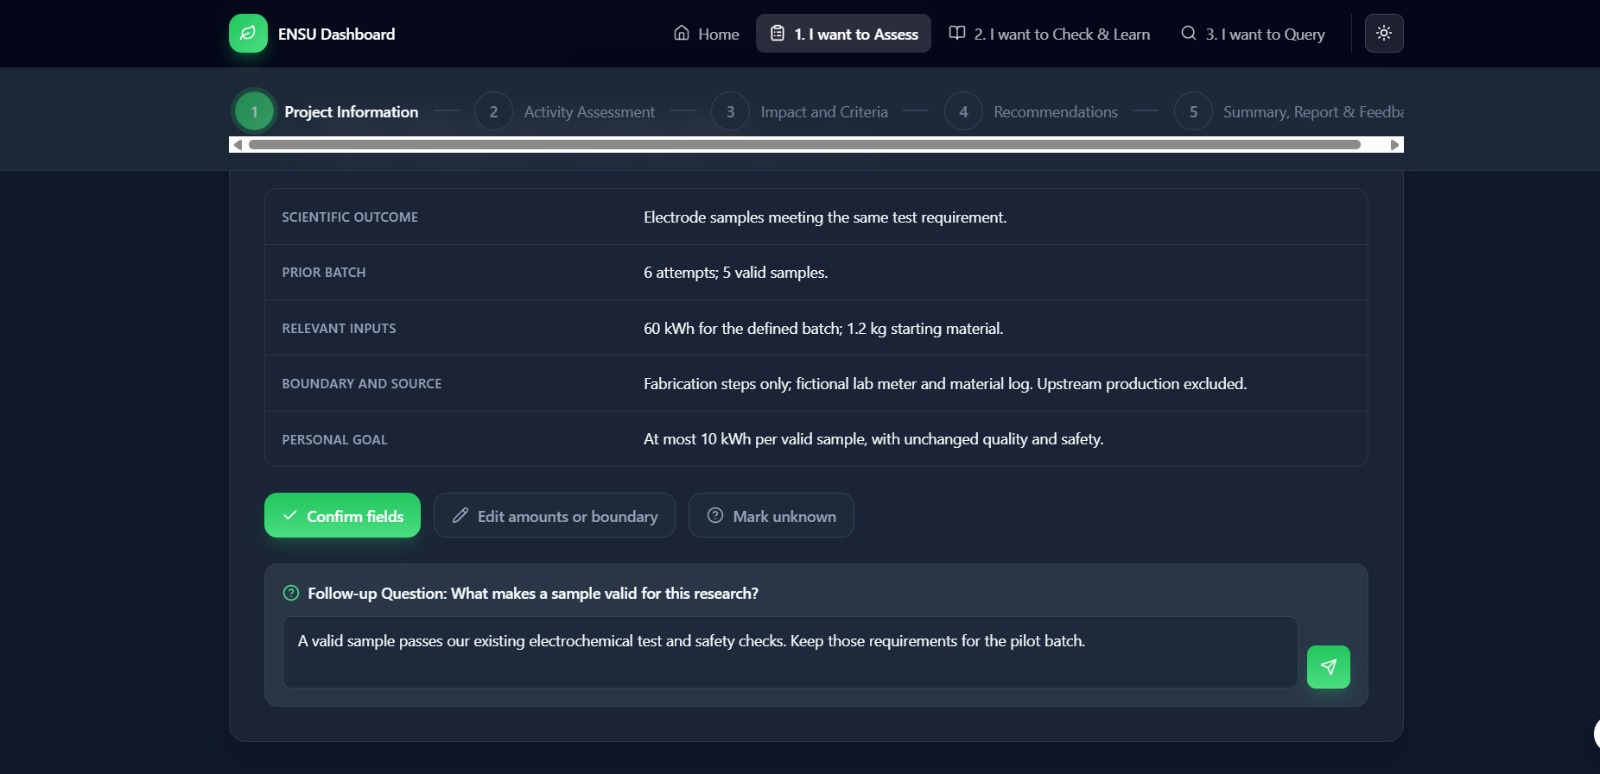
\includegraphics[width=\linewidth]{LaTeX_tuemscthesis2021/4.jpeg}
        \caption{I want to assess - project information}
    \end{subfigure}
    \hfill
    \begin{subfigure}{0.48\linewidth}
        \centering
        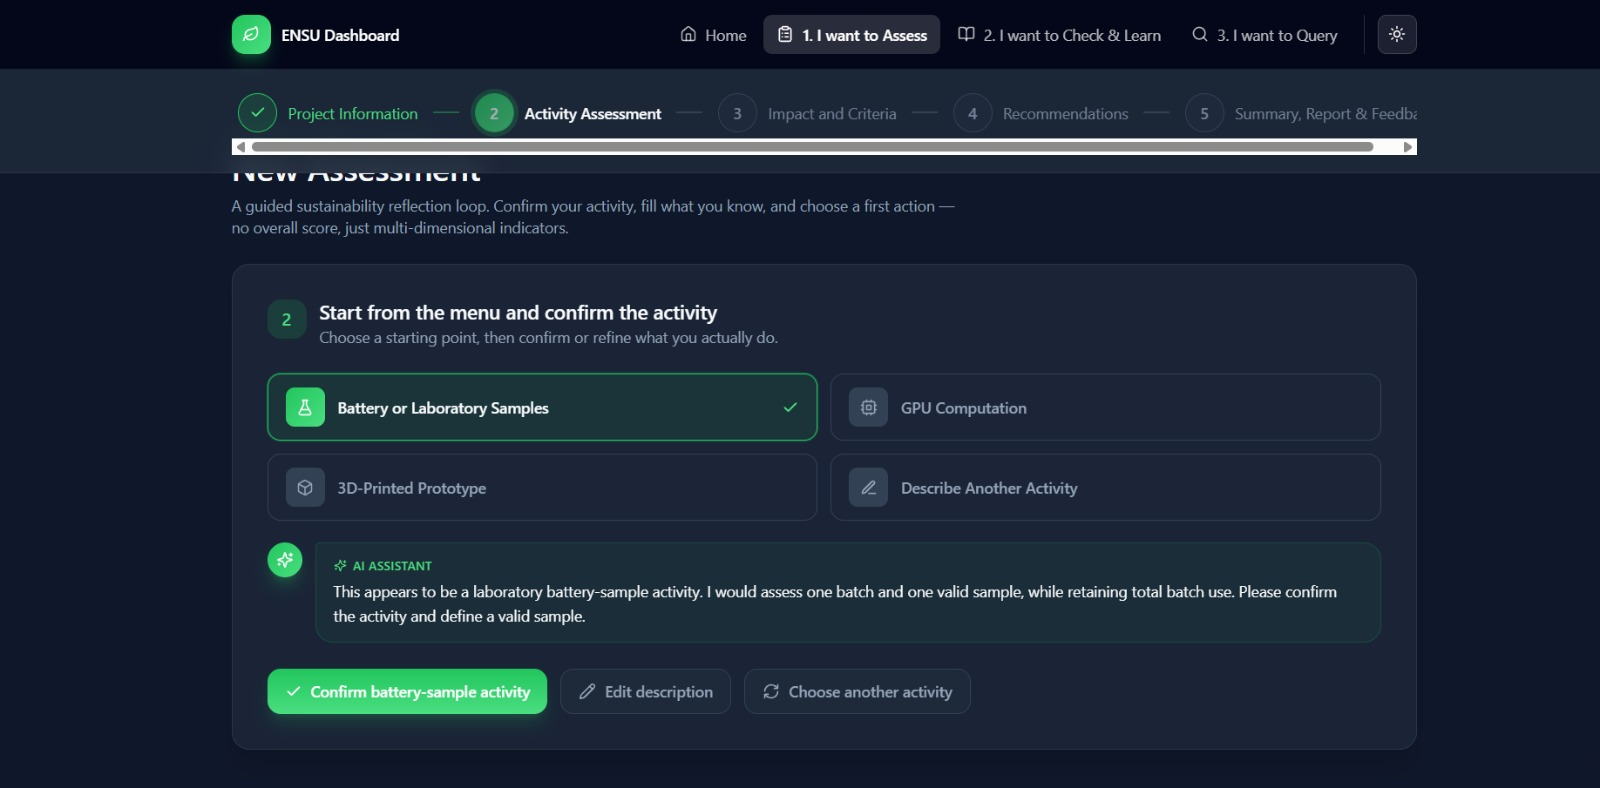
\includegraphics[width=\linewidth]{LaTeX_tuemscthesis2021/3.jpeg}
        \caption{I want to assess - activity assessment}
    \end{subfigure}
    
    \vspace{0.3cm}

    % Row 3
    \begin{subfigure}{0.48\linewidth}
        \centering
        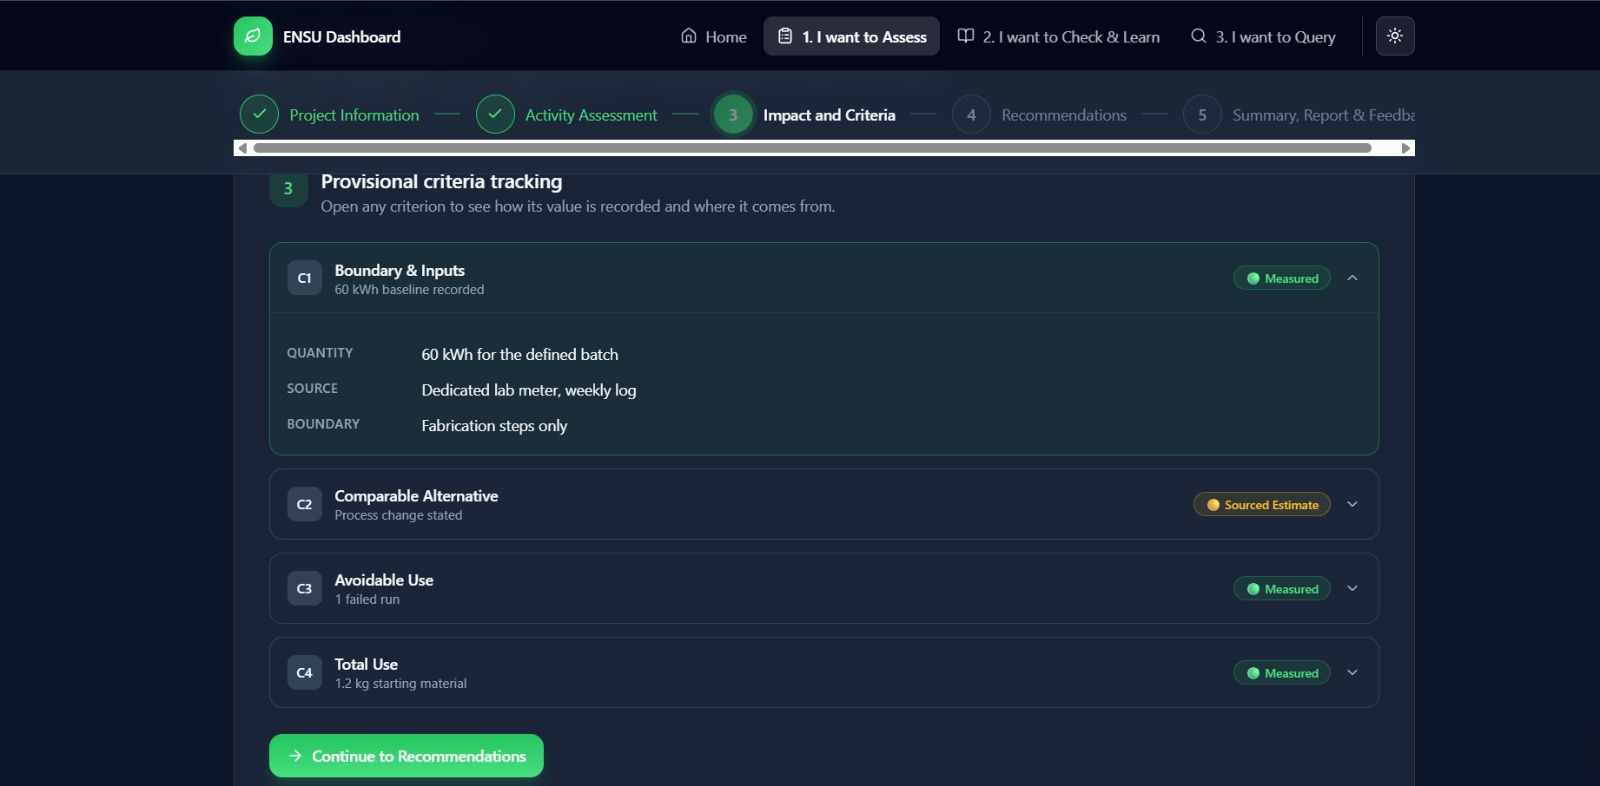
\includegraphics[width=\linewidth]{LaTeX_tuemscthesis2021/5.jpeg}
        \caption{I want to assess - impact and criteria}
    \end{subfigure}
    \hfill
    \begin{subfigure}{0.48\linewidth}
        \centering
        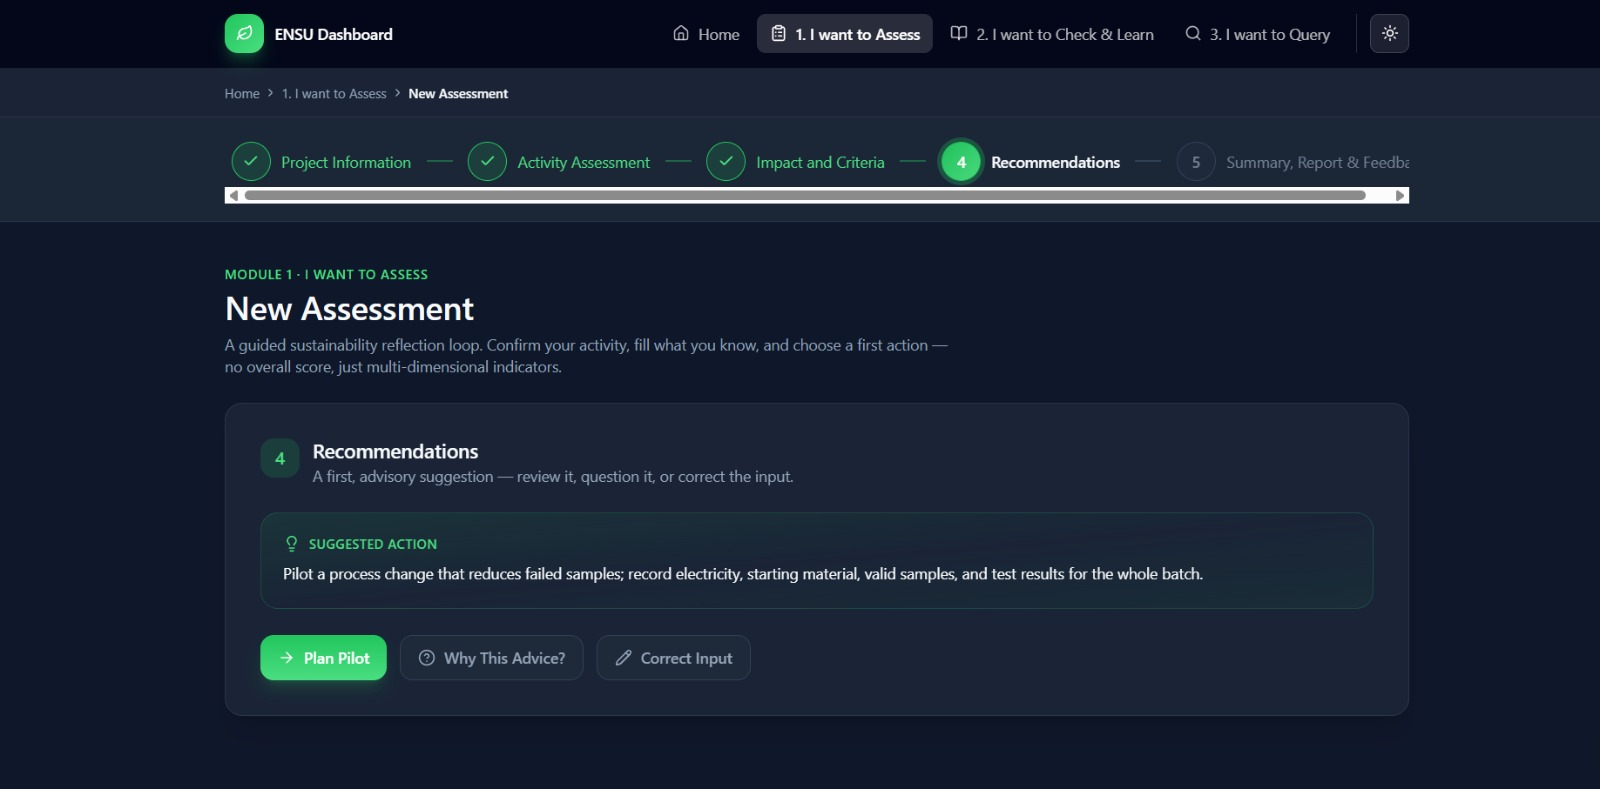
\includegraphics[width=\linewidth]{LaTeX_tuemscthesis2021/10.jpeg}
        \caption{I want to assess - recommendations}
    \end{subfigure}
    
    \vspace{0.3cm}

    % Row 4
    \begin{subfigure}{0.48\linewidth}
        \centering
        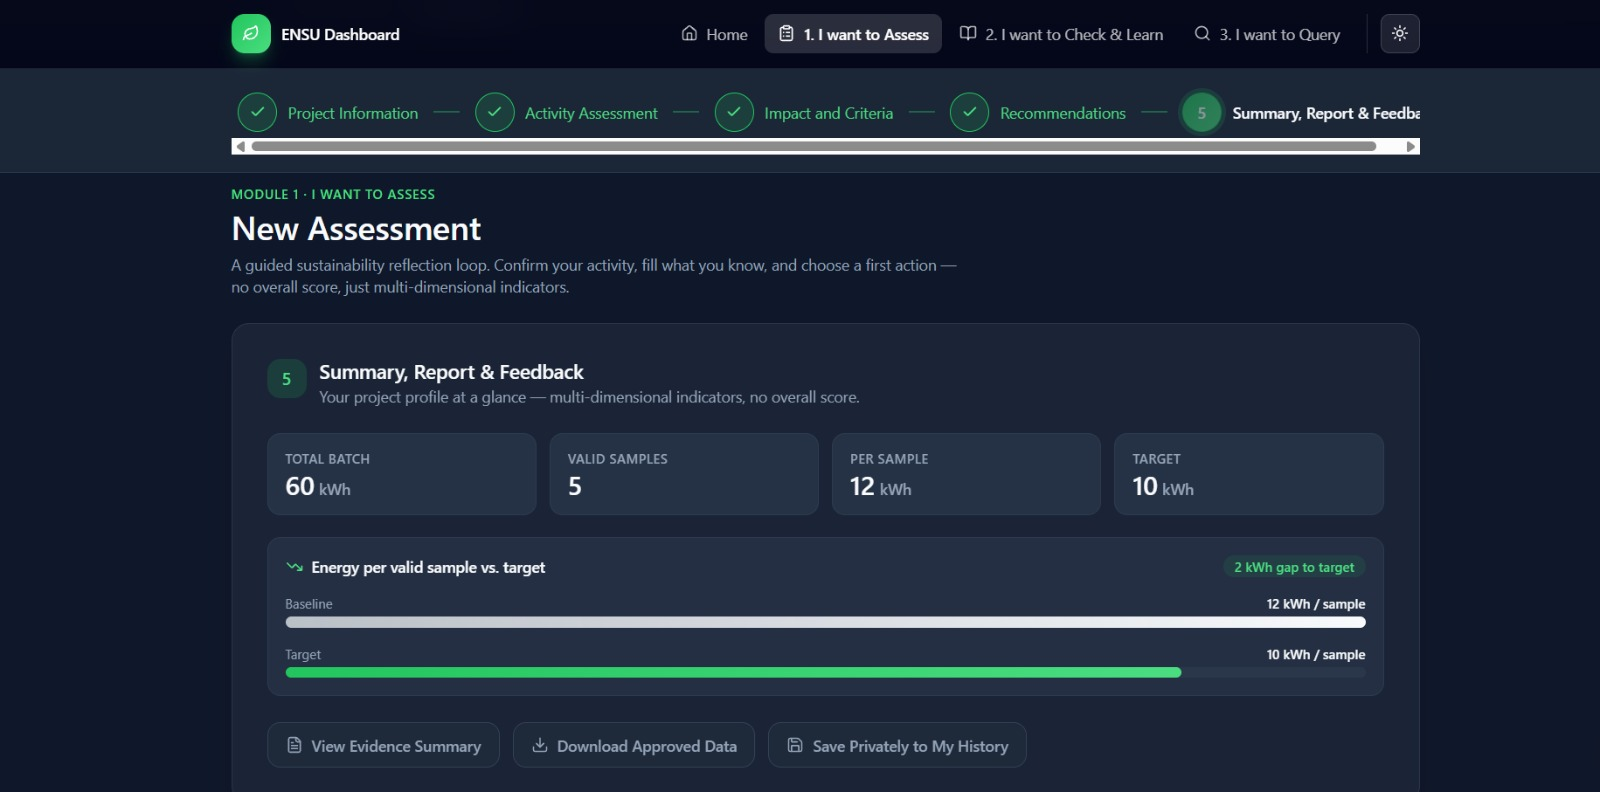
\includegraphics[width=\linewidth]{LaTeX_tuemscthesis2021/9.jpeg}
        \caption{I want to assess - summary, report \& feedback}
    \end{subfigure}
    \hfill
    \begin{subfigure}{0.48\linewidth}
        \centering
        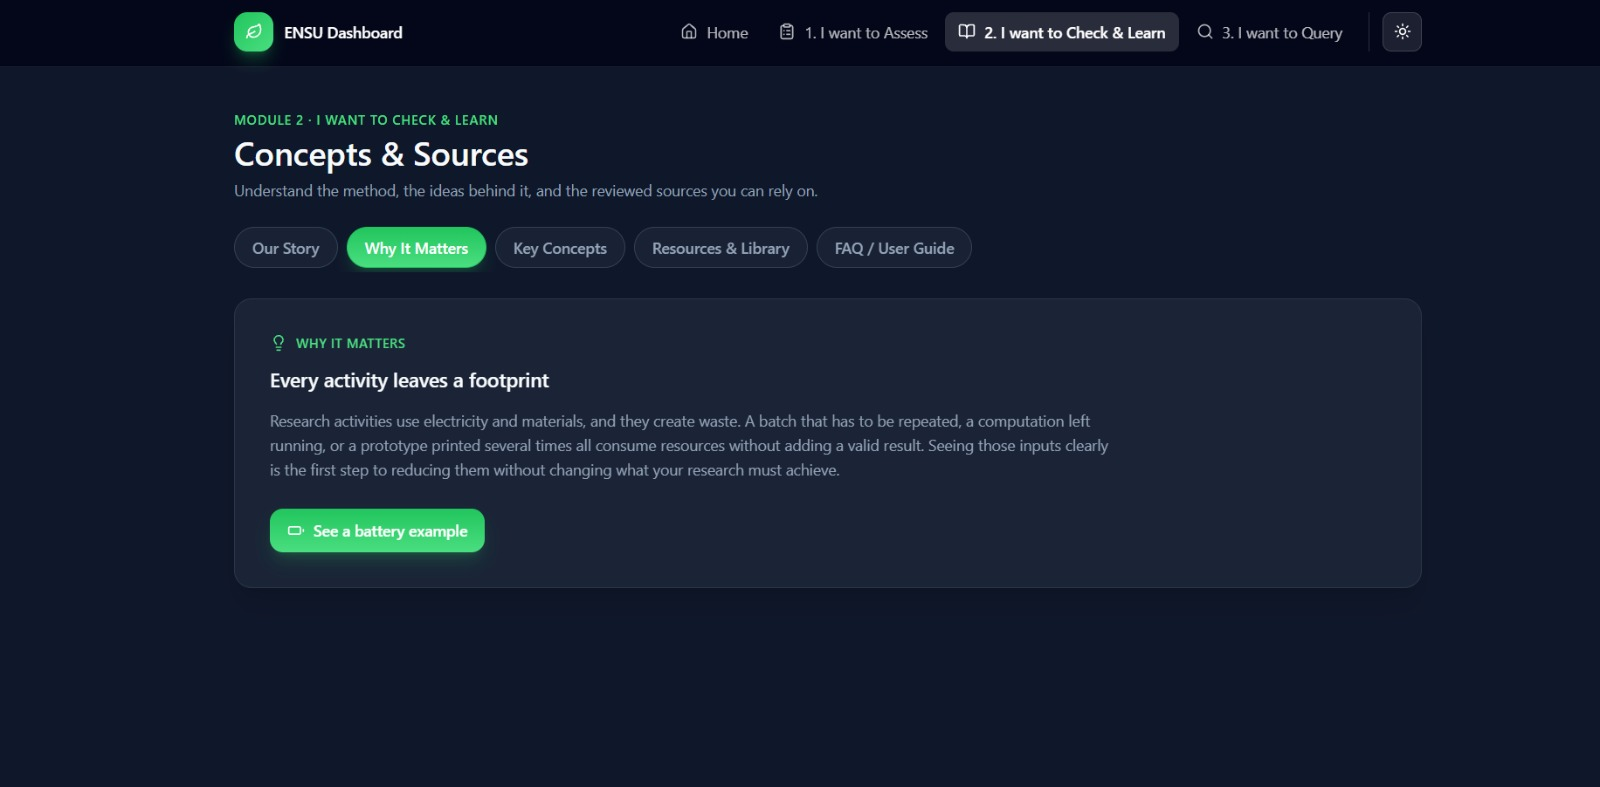
\includegraphics[width=\linewidth]{LaTeX_tuemscthesis2021/8.jpeg}
        \caption{I want to check and learn}
    \end{subfigure}

    \vspace{0.3cm}

    % Row 5
     \begin{subfigure}{0.48\linewidth}
        \centering
        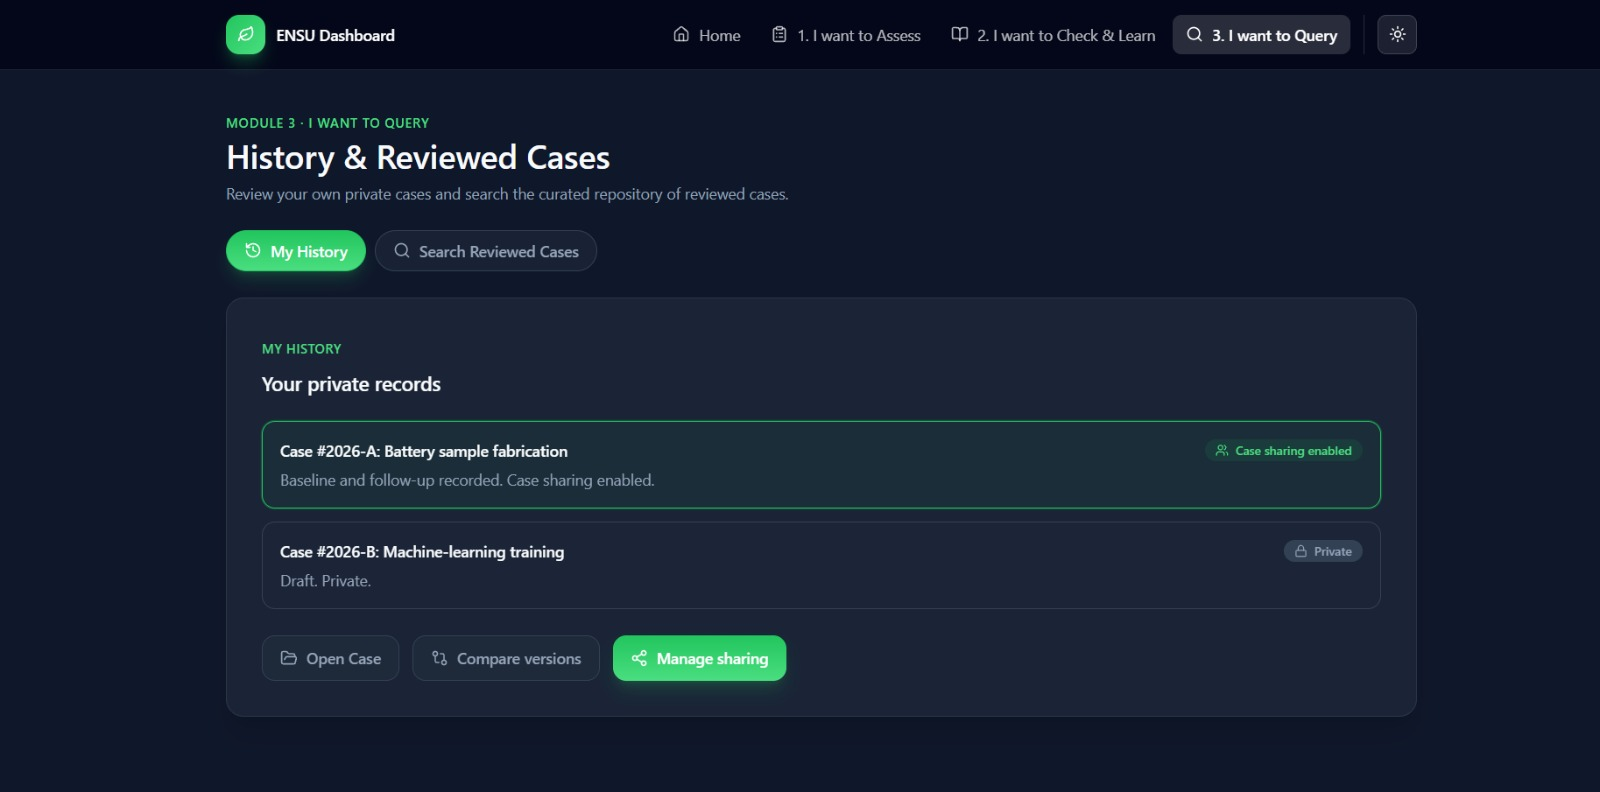
\includegraphics[width=\linewidth]{LaTeX_tuemscthesis2021/7.jpeg}
        \caption{I want to query - dark mode}
    \end{subfigure}
    \hfill
    \begin{subfigure}{0.48\linewidth}
        \centering
        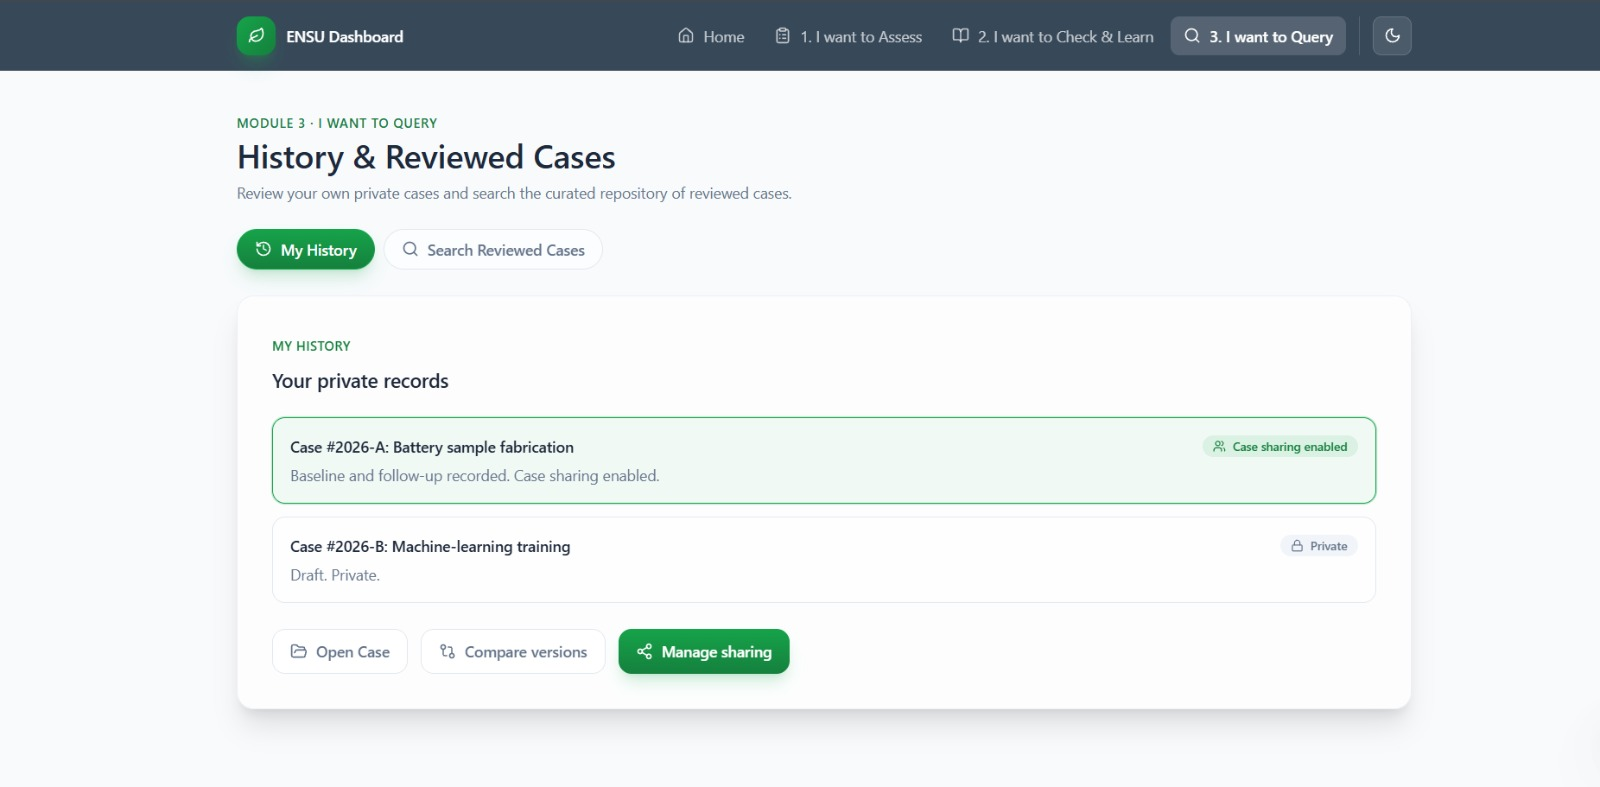
\includegraphics[width=\linewidth]{LaTeX_tuemscthesis2021/6.jpeg}
        \caption{I want to query - light mode}
    \end{subfigure}

    \caption{Complete Visual Representation of Our System}
    \label{fig:all_mockups}
\end{figure}
    \centering
    % Replace 'mockup-placeholder.png' with your exported UI screenshot file name
    % \includegraphics[width=0.9\textwidth]{mockup-placeholder.png} 
    \vspace{4cm} % Temporary spacing spacer for placeholder box
    

\clearpage

% =========================================================================
% H. TECHNICAL DOCUMENTATION & INSTRUCTIONS
% =========================================================================
\section*{H. Documentation of Prompts, Sources, and Tools}
\addcontentsline{toc}{section}{H. Documentation of Technical Tools}
\textit{Provide step-by-step instructions detailing the prompts, database registries, and tools explored, serving as a functional onboarding guide for future project hand-offs.}

\subsection*{Prompt Engineering Registry}
\begin{enumerate}
    \item \textbf{System Generation Prompts:} ...
    \item \textbf{Refinement & Interaction Queries:} ...
\end{enumerate}

\subsection*{Technical Infrastructure Setup}
[Document technical details like Streamlit/Gradio environments, database stacks, or UI component generators.]

% =========================================================================
% APPENDIX / REMINDERS FOR SEPARATE SUBMISSIONS (Optional Section)
% =========================================================================
\iffalse
\section*{Separate Evaluation Deadlines (Do Not Include in Main Paper PDF)}
The following elements are tracked by the course syllabus but must be submitted through their individual portals independently:
- I. Video/Oral Pitch (3-5 minutes)
- J. Personal Reflection (500 words per student)
- K. Peer Evaluation Sheet
\fi

\end{document}
In the responsible innovation statement we will assess our tool on different ethical principles. The use of AI raises concerns in terms of transparency, bias and reliability. We will discuss these concerns and provide measures to make sure our tool is in line with the users’ values. 

The first concern is the transparency of the tool. From the users perspective they submit their research into the tool and receive potentially previous done research on their topic. The user does not always know why the sources provided are relevant and whether the information provided by the AI is correct. The following measures will be taken:
Source transparency: Every source provided by the tool will need to include title authors year of publication the link to the original source and additional information if possible. This way the researches can verify the sources instead of having to trust the AI
Explanation of relevance: For each source provided a short explanation needs to be included on why the source was provided by showing similarities in research questions, methods etcetera. 

Depending on the available sources the Ai can be a bit biased. Especially if it only has access to certain types of sources like journals or only English sources. This could result in researchers missing previously conducted research when the tool does not have access to these sources. Our tool will try to prevent the bias as much as possible with the following measures: 
Database coverage: it should be clear for the user which databases the tool has access to. This way the user knows the limitations of the tool.
Search strategies: If possible the AI should make a broad search by using synonyms, interdisciplinary similarity and different terminology. 
User input: The user should be able to adjust the search query if they feel like it could be improved giving them more control over the results in case the AI runs into limitations. 

Our main design is to make it easy for the users to interpret the results by having a chatbot that provides the sources and explains why the sources are relevant. In future work we could help researches by providing improvements on their research. Even when there is research on the same topic there are still ways to differentiate. This way the researcher does not have to scrap everything and still conduct useful research. The tool could provide a better use of the resources for the research in case this happens. 
